\documentclass[11pt, a4paper]{article}
\usepackage[utf8]{inputenc}
\usepackage[slovak]{babel}
\usepackage[a4paper, text={17cm, 24cm}, left=2cm, top=3cm]{geometry}
\usepackage{graphicx} % Required for inserting images
\usepackage{listings}
\usepackage{subfigure}
\usepackage{xcolor}
\usepackage{amsthm}
\usepackage{amsmath}
\usepackage{float}
\graphicspath{ {./pics/} }
\lstdefinestyle{mystyle}{
    backgroundcolor=\color{black},  % Background color
    basicstyle=\color{white}\ttfamily, % Font color and style
    frame=none,              % No frame around code
    numbers=none,            % No line numbers
    showstringspaces=false,  % Don't show spaces in strings
    breaklines=true,         % Wrap long lines
    tabsize=4                % Tab size
}
\lstset{style=mystyle}
\begin{document}

\begin{titlepage}
\begin{center}
\Huge\textsc{Vysoké učení technické v~Brně\\
\huge{Fakulta informačních technologií}}\\
\vspace{\stretch{0.382}}
\Huge Používateľský manuál\\[0.5em]
\huge DIY Calculator\\
\vspace{\stretch{0.618}}
\end{center}
{\Large {2023/2024 \hfill Don't IVS yourself}}
\end{titlepage}
\newpage 

\tableofcontents

\newpage 

\section{Orientácia v prostredí}
\subsection{Rozloženie}

\begin{figure}[h]
    \centering
    \includegraphics{pics/Obrázok3.jpg}
    \caption{Rozloženie tlačidiel}
    \label{fig:enter-label}
\end{figure}

\section*{Obecná funkčnosť}

Aplikácia spracováva zadané čísla postupne a medzivýsledky vypisuje na displej. Ďalšie operácie teda počítajú s medzivýsledkom z predchádzajúcich výpočtov. Nepočíta sa teda s uprednostňovaním niektorých matematických operácií.

\textbf{Napr.} $1 + 2 \times 3 = 3 \times 3 = 9$
\begin{enumerate}
    \item \textbf{Nápoveda}\\
    Pre zobrazenie nápovedy stlačte tlačidlo '?' alebo klávesu 'H'.
    
    \item \textbf{Displej}\\
    Na prvom riadku sa zobrazí zadané číslo a po stlačení operácie sa zobrazí jej výsledok.
    
    Na druhom riadku sa zobrazuje celý zadaný reťazec čísel a operácií až po stlačení tlačidla '='.
    
    \item \textbf{Tlačidlo AC}\\
    Umožňuje zmazať výpočet, je možné použiť klávesu 'A'.
    
    \item \textbf{Pokročilé operácie}
    \begin{itemize}
        \item Ans - uloží výsledok z predchádzajúceho výrazu a použije ho v novom výraze. Je možné použiť klávesu 'A'.
        \item +/- - zmení znamienko zadaného čísla (napr. z čísla '10' urobí '-10'). Použitie: zadajte číslo a potom stlačte tlačidlo '+/-', je možné použiť klávesu 'G'.
        \item 1/x - preklopí hodnotu zadaného čísla (napr. z čísla '4' urobí '0.25'). Použitie: zadajte číslo a potom stlačte tlačidlo '1/x', je možné použiť klávesu 'I'.
        
        \item $x^2$ - umocní číslo dvoma, operácia berie jeden argument (je možné ju použiť niekoľkokrát za sebou, napr. $2^{2^2}$= 16 ). Je možné použiť klávesu 'S'.
        \item $x^n$ - umocní číslo n, operácia berie dva argumenty. Použitie: prvý operand je číslo, druhý je exponent. Je možné použiť klávesu 'E'.
        \item $\sqrt{x}$ - vypočíta druhú mocninu, operácia berie jeden argument (je možné ju použiť niekoľkokrát za sebou, napr. $\sqrt{\sqrt{16}} = 2$). Je možné použiť klávesu 'Q'.
        \item $^n\sqrt{x}$ - vypočíta n-tú mocninu, operácia berie dva argumenty. Použitie: prvý operand je číslo, druhý je mocnina. Je možné použiť klávesu 'R'.
        \item \% - modulo, operácia berie dva argumenty. Použitie: prvý operand je číslo, druhý je deliteľ. Je možné použiť klávesu '\%'.
        \item $|x|$ - absolútna hodnota, operácia berie jeden argument. Použitie: urobí absolútnu hodnotu z celého výrazu, pred stlačením tlačidla '$|$x$|$. Je možné použiť klávesu 'B'.
        \item $x!$ - faktoriál, operácia berie jeden argument (je možné ju použiť niekoľkokrát za sebou, napr. $3!! = 720$). Je možné použiť klávesu '!'.
    \end{itemize}
    
    \item \textbf{Základné operácie}\\
    Binárne operácie násobenie, odčítanie, násobenie, delenie. Je možné použiť klávesy '+', '-', '*' a '/'.
    
    \item \textbf{Čísla}\\
    Pre zadávanie čísel je možné použiť klávesy '0'-'9'.
    
    Pre zadanie desatinnej čiarky je možné použiť klávesy '.' a ','.
    
    \item \textbf{Rovná sa}\\
    Vypíše výsledok pre celý výraz a uloží ho (pre opätovné použitie), je možné použiť kláves '='.
\end{enumerate}
\newpage
\subsection{Ovládanie pomocou kláves}
\begin{table}[H]
\begin{center}
\begin{tabular}{|c|c|}
\hline
\textbf{Klávesa} & \textbf{Hodnota}     \\ \hline
'0-9'            & 0-9                  \\ \hline
'H'              & Nápoveda             \\ \hline
'.'              & Čiarka               \\ \hline
','              & Čiarka               \\ \hline
'+'              & Plus                 \\ \hline
'-'              & Mínus                \\ \hline
'*'              & Násobenie            \\ \hline
'/'              & Delenie              \\ \hline
'\%'             & Percento             \\ \hline
'S'              & Druhá mocnina        \\ \hline
'E'              & Mocnina n-tého čísla \\ \hline
'Q'              & Druhá odmocnina      \\ \hline
'R'              & N-tá odmocnina      \\ \hline
'!'              & Faktoriál            \\ \hline
'='              & Rovná sa             \\ \hline
'A'              & Výsledok             \\ \hline
'C'              & Vynulovať            \\ \hline
\end{tabular}
\end{center}
\end{table}
\subsection{Výnimky}
\begin{itemize}
 \item Pri delení 0 sa vypíše na obrazovku Error.
 \item Pri dosiahnutí maxima mocniny sa vypíše nekonečno (inf).
 \item Pri presiahnutí maximálneho faktorialu (164!) sa vypíše Error. 
\end{itemize}

\newpage
\section{Inštalácia}
V inštaláčnom balíčku je taktiež obsiahnutý spustiteľný súbor na výpočet smerodajnej odchýlky spolu s kalkulačkou. Na celkovo inštaláciu stačí mať \textbf{calculator-1.0-Alpha-Linux.deb} a \textbf{preinstal.sh}.
\subsection{Inštalácia pomocou príkazov}
Príkaz na skopírovanie repozitára z \textbf{githubu}. Ak užívateľ nemá nainštalovaný git v zariadení, je nutná inštalácia gitu predom: \\  
\verb|$    sudo apt-get install git |  \\
\verb|$    git clone --recursive https://github.com/H0CK3Y03/dont_ivs_yourself.git |  \\ \\
V prípade chýbajúcich závislostí je nutné predom spustiť skript, ktorý doinštaluje všetko potrebné a rovno spustí inštaláciu balíčka. Je nutné priradiť skriptu práva na spustenie: \\ 
\verb|$    chmod +x preinst.sh| \\ \\
Súbory \textbf{calculator-1.0-Alpha-Linux.deb} a \textbf{preinstal.sh} je nutné mať v jednom adresári. \\
\verb|$    ./preinstal.sh| \\ \\
Samostatná inštalácia balíčka: \\
\verb|$    sudo dpkg -i ./calculator-1.0-Alpha-Linux.deb| \\
\newpage
\subsection{Inštalácia pomocou inštalačného balíčku}
\textbf{Obr.1:} Po následnom stiahnutí balíčka, pravým tlačidlom klikneme na ikonu balíčka. 
\begin{figure}[H]
    \centering
    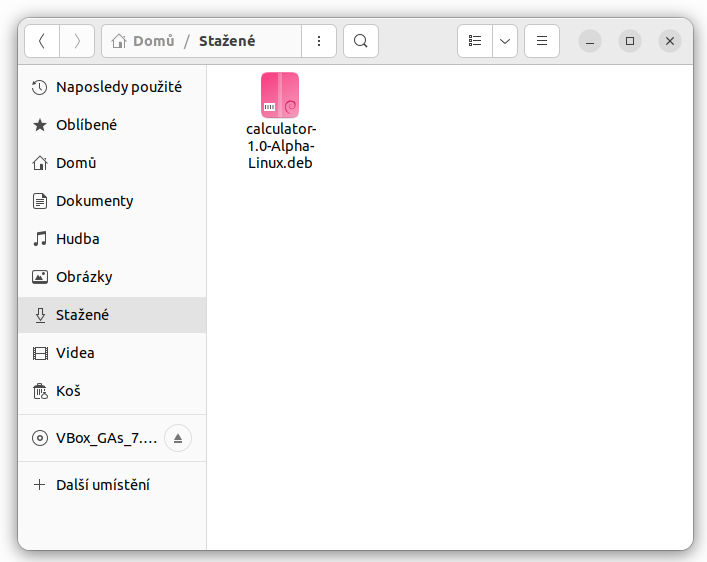
\includegraphics[width=0.5\textwidth]{1.png} 
    \label{fig:i1} 
\end{figure}
\noindent \textbf{Obr.2:} Zvolíme možnosť 'Otevřít jinou aplikaci'
\begin{figure}[H]
    \centering
    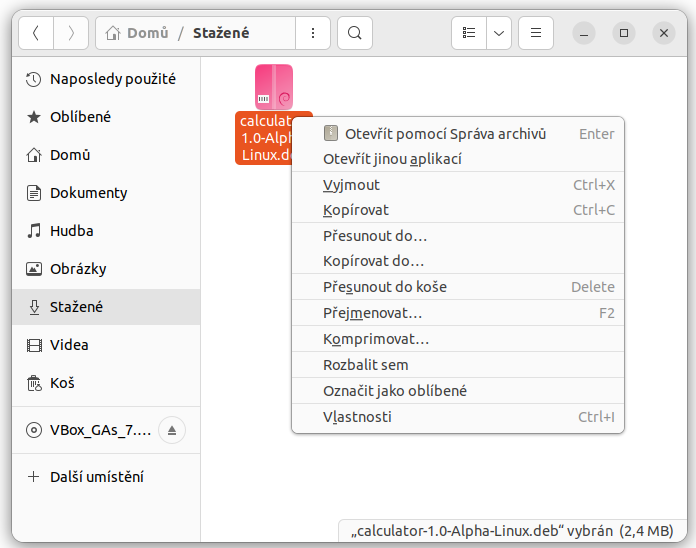
\includegraphics[width=0.5\textwidth]{2.png}
    \label{fig:i2}
\end{figure}
\newpage
\noindent \textbf{Obr.3:} Tu si zvolíme 'Instalace softwaru'
\begin{figure}[H]
    \centering
    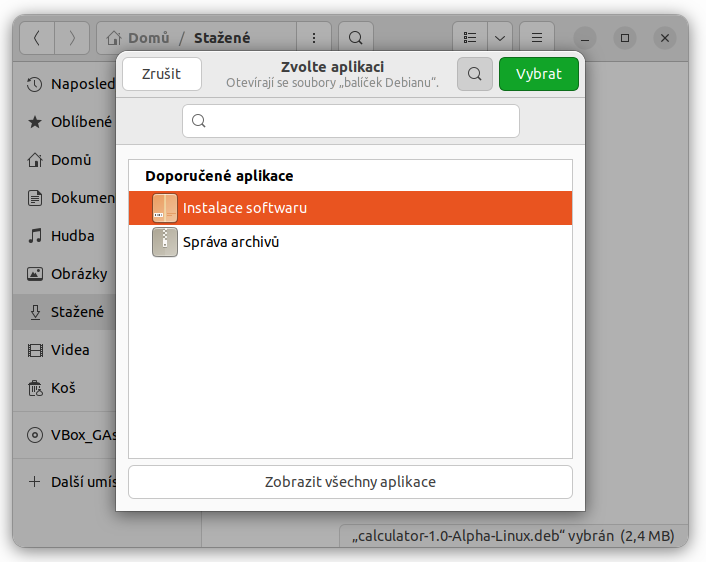
\includegraphics[width=0.5\textwidth]{3.png}
    \label{fig:i3}
\end{figure}
\noindent \textbf{Obr.4:} Po kliknutí na zelené tlačidlo 'Instalovat', sa spustí inštalácia.
\begin{figure}[H]
    \centering
    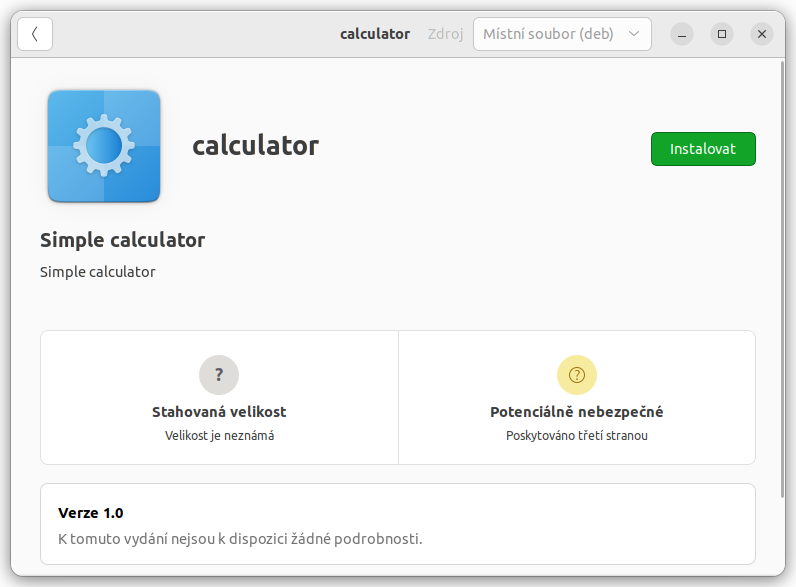
\includegraphics[width=0.5\textwidth]{4.png}
    \label{fig:i4}
\end{figure}
\noindent \textbf{Obr.5:} Následne sa vám po nainštalovaní zobrazí ikonka medzi aplikaciami. 
\begin{figure}[H]
    \centering
    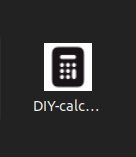
\includegraphics[width=0.2\textwidth]{5.png}
    \label{fig:i5}
\end{figure}

\newpage
\section{Odinštalácia}
\subsection{Odištalácia pomocou príkazov}
\verb|$    sudo apt remove calculator| \\
\subsection{Odištalácia pomocou inštalačného balíčku}
\textbf{Obr.1:} Odinštaláciu spustíme dvojklikom alebo pomocou inštalačného balíčka, kde zvolíme rovnaký postup ako na inštaláciu. Po kliknutí na červené tlačidlo vyskočí okno s upozornením. Odinštalácia sa spustí až po zakliknutí červeného tlačidla 'Odinstalovat'.
\begin{figure}[ H]
    \centering
    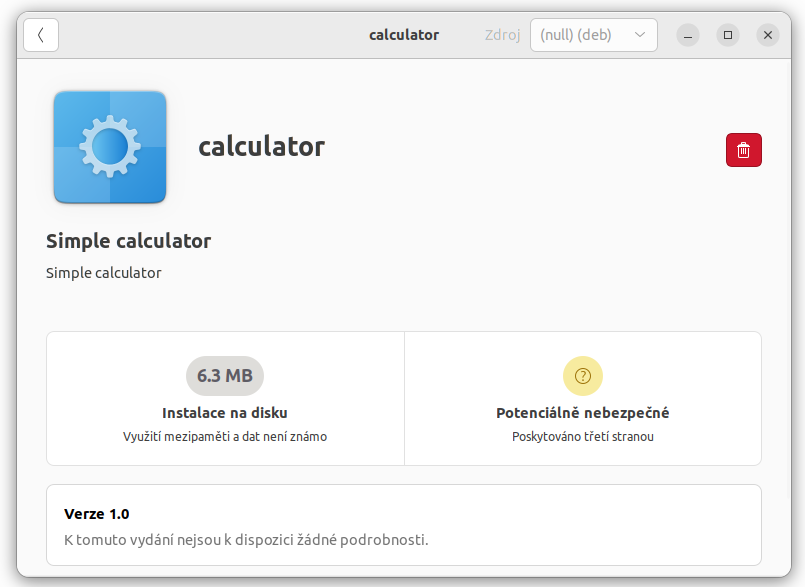
\includegraphics[width=0.5\textwidth]{u1.png}
    \label{fig:u1}
\end{figure}

\section{Smerodajná odchýlka}
Pomocou príkazu \verb|stddev| spustíte výpočet smerodajnej odchýlky. Spustenie vo formáte \verb|stddev| vám dovolí písať hodnoty rovno do terminálu, pomocou stlačenia Ctrl + D sa uložia hodnoty. Spustenie vo formáte \verb|stddev < hodnoty.txt| vtedy sa výpočet rovno vypíše (hodnoty.txt môže byť nahradený za váš súbor). \\ \\
\textbf{Formát pre písanie vlastných hodnôt rovno do terminálu pre výpočet:} \\
\verb|$   stddev| \\
\verb|[ukončenie Ctrl + D]| \\ \\
\textbf{Formát pre vloženie pripraveného súboru na výpočet:} \\
\verb|$   stddev < hodnoty.txt|
\end{document}
